\chapter{Identification}
    The purpose of Identification is to perform actions that can fall anywhere in computer science.\\
    We'll look at either the methodologies and specific forensics cases.\\
    Tipically we use Linux:
    \begin{itemize}
        \item extensive native file system support 
        \item we can just dump a disk image as a file with linux, and we can mount the copy as if it were a drive, also read only to prevent writing and keep the copies not touched.
    \end{itemize}
    Why not Windows? Nobody uses windows by itself. It must be confined, it stinks.
    \begin{itemize}
        \item It tampers with drives by automatically mounting them and writing on them.
        \item No image handling or hotswapping of drives.
        \item No support for non Windows filesystems.
    \end{itemize}
    The best thing to do is to use linux as host with windows as guest on virtual machines:
    \begin{itemize}
        \item Work the images with Linux, mount them read-only and exporting them via Samba or vmware \textit{"not persistent"} to Windows.
        \item Use specific windows tools
    \end{itemize}
    Keep in mind that sharing something like this, is doing it file level: any utility that analize drives cannot work in this way.
    \subsection{What does scientific mean?}
        We defined scientific as repeatable. Any other expert will be able to perform the same experiment, on a clone of the image, obtaining the same results I obtained.\\
        The experiment is not just a black box tool with an input and an output, the expert must be able to perform the same analysis by hand (at least in theory). This means that analysis software needs to be open sourced, and possibly free. Proprietary or "law enforcement only" tools can be used but the analysis must be performed again with something repeatable. \textit{(Judges, Lawyers, Marescialli, they can access the source for "law enforcement only" tools)}.
    \subsection{What does analyisis mean?}
        During the analysis phase, we may need to apply many techniques from computer science, that's the reason because people goes to a forensic expert. 
        Forensic experts are able to do analysis because they are competent in computer science in general. They can also be ethically prone to call other experts in fields in which they're not so expert.
    \section{Recovery of deleted data} 
        Data/evidence may have been voluntarily or unvoluntarily deleted because time passed, because of the OS, because the drive was formatted, because the drive was faulty.
        In many of these cases, we may be able to reconstruct all or part of the information, which is one of the most typical tasks computer forensics experts perform.\\
        Let's look at the UNIX file system again for the millionth time to recall basic elements on data storage by OSs:\\
        \begin{figure}
            \centering
            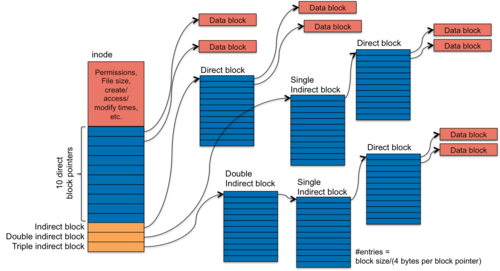
\includegraphics[width=0.7\linewidth]{filesystem.png}
        \end{figure}
        A file system is a way to organize the space on a drive to store information. It's an archive-like thing.
        The basic idea is to have units of information \textit{(files)}, to put on the storage drive, and then to have an index of what is stored and where. Following the index I can find the place where things are stored.\\
        Whithout the index I may not reach them \textit{(if they were deleted)} but they can still be stored:\\
        when we delete a file the operating system just marks the file as deleted and just doesn't shows it no more. The actual data will go away when overwritten by other files.\\
        Indexes and data will go away randomly and independently from each other, statistically on a large hard drive there is a good possibility that metadata goes away before data blocks.
        \subsection{Disk Geometry}
            tracks, cylinders \dots 
            \begin{figure}
                \centering
                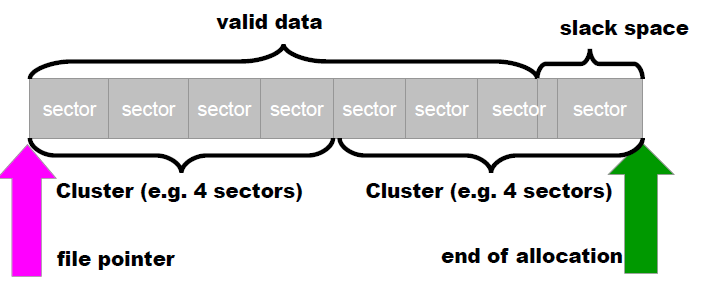
\includegraphics[width=0.7\linewidth]{sectors.png}
            \end{figure}
            When reading and writing, the minimum portion of a track is called sector, each drive has a different sector size, and the OS can't manage it for each of the existent models.\\
            OS's filesystems are made to work on clusters of sectors \textit{(NTFS uses 4kb clusters)}, independently of the real dimension on the drive. So, storing for example a file of size 5kb needs 1 cluster of 4kb + a fourth of a cluster, and leaves the remaining part as unused slack space.\\
            In the slack space there can possibly be remainances of old files, obviously they can be small portions, so only small files can be retrieved \textit{(e-mails, text files \dots)}, while other filetypes can't because they need to be full to be read \textit{(images, encrypted files \dots)}\\
            Sectors are one after the other, if we place a file on a drive there is a good possibility that all the sectors of it are one after the other, so by scanning \textit{(cramming)} the drive can be possible to find them and restore them too.\\
            The issues are with fragmented files, it was a big problem on small drives, now in most cases drives are so large to not fragment and most of OS's try to not break files for performance reasons. There still are techniques to find fragments of files and restore them.\\
            Another issue is with encrypted, compressed files. In those cases we really need the file to be complete to be able to read them.\\
            Headerless files because they were taken away header or footer cannot be interpreted. Headerless compressed/encrypted files are unpracticable.
        \subsection{Free software tools for data recovery}
            \begin{itemize}
                \item TSK and Autopsy can perform data recovery under linux, they support NTFS, FAT, FFS, EXT2, EXT3..
                \item Foremost can perform file recovery trough carving
                \item gpart, testdisk can perform partition recovery
                \item photorec can seek specifically for images or videos
            \end{itemize}